\documentclass{article}

\usepackage{tocloft}
\usepackage[top=2.5cm, bottom=2.5cm, left=2.2cm, right=2.2cm]{geometry}
\usepackage{graphicx}
\usepackage{amsmath}
\usepackage[localise,Kashida]{xepersian}

\renewcommand{\cftsecleader}{\cftdotfill{\cftdotsep}}
\settextfont[
  Path=fonts/,
  UprightFont = *-Regular,
  BoldFont = *-Bold,
  ItalicFont = *-Variable
]{Vazir}

\begin{document}

\setLTRbibitems{}

\نویسنده{الهه داستان}
\عنوان{طراحی و پیاده‌سازی سیستم پیش‌بینی ترافیک بر پایه شبکه‌های عصبی}
\تاریخ{\امروز}
\عنوان‌ساز
\فهرست‌مطالب

\قسمت{فرم تعریف پروژه}

\شروع{جدول}{|p{\textwidth}|}

\خط‌پر
عنوان پروژه: طراحی و پیاده‌سازی سیستم پیش‌بینی ترافیک بر پایه شبکه‌های عصبی\\
\خط‌پر
استاد راهنما‌ی پروژه:‌ دکتر رضا صفابخش \پرا امضا \\[0.5cm]
\خط‌پر
مشخصات دانشجو:
\شروع{توضیح}
\فقره[نام و نام‌خانوادگی] الهه داستان
\فقره[شماره دانشجویی] ۹۶۳۱۰۲۵
\فقره[ترم ثبت پروژه] نیمسال دوم ۱۳۹۹ - ۱۴۰۰
\پایان{توضیح}\\
\خط‌پر
داور پروژه:‌ دکتر محمد رحمتی \پرا امضا \\[0.5cm]
\خط‌پر
در این پروژه قصد داریم ترافیک را در شبکه‌ای از خیابان‌ها و چهارراه‌ها با استفاده از وابستگی‌های زمانی و مکانی‌پیش‌بینی
کنیم. برای اینکار به جای استفاده از روش‌های سنتی که کارآیی خوبی نداشته‌اند از پیچش روی گراف‌ها بهره خواهیم جست. \\
\خط‌پر
وسائل مورد نیاز:
\شروع{فقرات}
\فقره امکان دسترسی به مقالات
\فقره یک سرور جهت اجرا و ارزیابی مدل‌ها (نیازمندی‌های سخت‌افزاری در پیوست آمده است)
\پایان{فقرات} \\
\خط‌پر
محل انجام پروژه:‌ دانشکده مهندسی کامپیوتر دانشگاه امیرکبیر \پرا تاریخ شروع: اسفند ۱۳۹۹ \\
\خط‌پر

\پایان{جدول}

\قسمت{تعریف مساله}
\پاراگراف{}
پیش‌بینی سرعت ترافیک برای کنترل و هدایت آن ضروری است.
به علت پیچیدگی و غیرخطی بودن سرعت ترافیک روش‌های قدیمی نمی‌توانند ترافیک را برای سفرهایی با زمان طولانی و متوسط به خوبی پیش‌بینی کنند.
پیش‌بینی دقیق و بی‌درنگ سرعت ترافیک برای افراد و سازمان‌های ارائه دهنده‌ی خدمات حمل و نقل و حتی دولت موضوع مهمی است چرا که حمل و نقل نقش مهمی در زندگی هر فرد ایفا می‌کند و یکی از اصلی‌ترین توانایی‌ها در سیستم ترابری هوشمند \پانویس{Intelligent Transportation System} به شمار می‌رود.
در این پروژه سعی داریم با استفاده از آموزش دادن شبکه‌های عصبی عمیق به پیش‌بینی سرعت ترافیک در برخی نقاط مشخص (مانند چهارراه‌ها و میدان‌ها) بپردازیم.
امروزه با استفاده از داده‌های عظیمی که در دسترس است و همچنین پیشرفت سخت‌افزار می‌توانیم شبکه‌های عمیقی که در گذشته قابل آموزش نبودند را آموزش دهیم و از توانایی بالای آن‌ها در پیش بینی مسائل پیچیده استفاده کنیم.

\قسمت{مرور پیشینه}
\پاراگراف{}
پیش‌بینی سرعت ترافیک بر مبنای طول سفر به دو دسته‌ی کلی کوتاه (۵ تا ۳۰ دقیقه) ‌و متوسط-طولانی (بیشتر از ۳۰ دقیقه) تقسیم می‌گردد. اکثر روش‌های آماری مانند رگراسیون خطی در سفرهای کوتاه مدت عملکرد خوبی دارند، اما به علت عدم قطعیت و پیچیدگی سرعت ترافیک این روش‌ها در سفرهای طولانی مدت دقت خوبی ندارند.~\مرجع{1709.04875}

\پاراگراف{}
مطالعات قبلی بر روی پیش‌بینی سرعت ترافیک در سفرهای بلند مدت را می‌توان به دو دسته‌ی مدل کردن پویا و روش‌های داده‌محور تقسیم کرد.
در روش‌های مدل کردن پویا از ابزار ریاضیاتی، مانند معادلات دیفرانسیل و دانش فیزیکی، برای فرموله کردن مسائل ترافیک استفاده می‌شود.~\مرجع{Vlahogianni2015}
در این روش برای رسیدن به حالت پایدار در پروسه‌ی شبیه‌سازی به سیستم‌های پیچیده و توانایی محاسباتی بسیار بالا نیاز است و فرضیه‌ها برای ساده‌سازی، دقت پیش‌بینی را کاهش می‌دهند.
به همین علت و همانطور که پیشتر بیان شد، به دلیل وجود داده‌ی زیادی که امروزه قابل دسترس است، علاقه به سمت روش‌های داده محور بیشتر است.
در روش‌های داده محور مدل‌های آماری کلاسیک و مدل‌های یادگیری ماشین دو نماینده‌ی اصلی هستند.

\پاراگراف{}
روش مدل خود همبسته میانگین متحرک\پانویس{Auto-Regressive Integrated Moving Average} و انواع آن یکی از روش های تجزیه و تحلیل سری زمانی است که مبتنی بر آمار کلاسیک\پانویس{Classical Statistics} است
و در طول زمان بسیار مورد بحث قرار گرفته است~\مرجع{Williams2003}،
اما این مدل محدود به فرضیات ثابتی درباره‌ی توالی‌های زمانی است و نمی‌تواند ارتباطات زمانی-مکانی را به حساب بیاورد.
اخیرا روش‌های یادگیری ماشین در پیش‌بینی سرعت ترافیک توانسته‌اند مدل‌های آماری کلاسیک را به چالش بکشند.

\پاراگراف{}
امروزه روش‌های یادگیری عمیق با موفقیت بر روی مسايل ترافیکی اعمال شده‌اند و پیشرفت‌های زیادی در این زمینه صورت گرفته است،
مانند شبکه‌ی باور عمیق\پانویس{Deep Belief Network}~\مرجع{YuhanJia2016} و کدکننده خودکار پشته‌ای\پانویس{Stacked Auto Encoder}~\مرجع{Chen_Song_Yamada_Shibasaki_2016}.
اما برای این شبکه‌های متراکم سخت است که بتوانند ویژگی‌های زمانی و مکانی را به طور مشترک از ورودی استخراج کنند.
همچنین در هنگام محدودیت و یا غیبت ویژگی‌های مکانی توانایی این شبکه‌ها تحت تاثیر قرار میگیرد.

\قسمت{راه‌حل پیشنهادی}

\پاراگراف{}
برای درک بهتر موضوع همزمان با توضیح راه‌حل یک مثال را به طور موازی پیش می‌بریم.

\پاراگراف{}
هدف از این پروپوزال بیان راه‌حلی برای پیش‌بینی سرعت ترافیک در برخی مختصات‌ها (مانند تعدادی میدان) در چند گام زمانی آینده است که
بدین جهت از سرعت ترافیک در این محل‌ها در گام‌های زمانی پیشین استفاده می‌کنیم. رابطه \رجوع{eq:base} این مساله سری زمانی را به زبان ریاضی توصیف می‌کند.

\begin{equation}
  \label{eq:base}
  \hat{v}_{t+1}, \ldots,  \hat{v}_{t+H} = \mathop{\mathrm{argmax}} \log \mathsf{P}({v}_{t+1}, \ldots,  v_{t+H} | v_{t-M+1} , \ldots,  v_{t})
\end{equation}

\begin{table}[h]
  \centering
  \caption{توضیح پارامترهای رابطه \رجوع{eq:base}}
  \begin{tabular}{|c|p{0.5\textwidth}|}
    \hline
    $v_{t}$ & یک بردار به طول تعداد نقاطی که قصد داریم سرعت ترافیک را در آن‌ها پیش‌بینی کنیم که هر المان شامل سرعت ترافیک در یکی از مختصات‌های مورد نظر در زمان $t$ است. \\
    \hline
    $\hat{v}_{t+1}$ & سرعت پیش‌بینی شده در زمان $t+1$ \\
    \hline
    $H$ & تعداد گام های زمانی آینده که می‌خواهیم سرعت ترافیک را پیش بینی کنیم. \\
    \hline
    $M$ & تعداد گام های زمانی پیشین که برای پیش بینی استفاده می‌کنیم. \\
    \hline
  \end{tabular}
  \label{tbl:base}
\end{table}

\پاراگراف{}
برای مثال فرض کنیم می‌خواهیم سرعت ترافیک را در میدان فاطمی و میدان فلسطین (دو میدان معروف در تهران) پیش‌بینی کنیم.
$v_{t}$ یک بردار به طول دو خواهد بود که یک عضو آن سرعت ترافیک در میدان فاطمی در زمان $t$ مانند ساعت دو بعد از ظهر امروز و عضو دیگر آن شامل همین اطلاعات برای میدان فلسطین خواهد بود.
در این مثال $H$ را برابر یک و $M$ را برابر سه در نظر می‌گیریم. منظور از \رجوع{eq:base} این است که قصد داریم سرعت ترافیک در $H$ قدم زمانی بعدی را با دانستن $M$ قدم زمانی قبلی پیش‌بینی کنیم.

\پاراگراف{}
برای پیش‌بینی سرعت ترافیک در نقاط مختلف از هر دو نوع ویژگی زمانی و مکانی بهره می‌بریم.
در روش‌های پیشین مانند \مرجع{1506.04214} از پیچش\پانویس{convolution} معمول که عمدتا در پردازش تصویر از آن بهره می‌گیرند استفاده شده است، این پیچش تنها می‌تواند بر روی داده‌هایی اعمال شود که ساختار مشبک دارند (مانند عکس و فیلم).
در این روش برای آنکه بتوانیم از اطلاعات مکانی حداکثر استفاده را ببریم به جای آنکه شبکه‌ی ترافیک را مانند یک شبکه‌‌ی شطرنجی\پانویس{Grid} ببینیم،
آن را به وسیله‌ی یک گراف مدل می‌کنیم و پیچش را مستقیما بر روی این گراف اعمال می‌کنیم.

\پاراگراف{}
گره‌های این گراف نقاطی مشخص هستند که سرعت ترافیک را در آن‌ها داشته باشیم، در این مثال نقاط ما میدان‌های فاطمی و فلسطین هستند،
سرعت در این نقاط به طور مثال می‌تواند از طریق دوربین‌های سرعت سنج یا از طریق سیستم موقعیت‌‌یاب‌جهانی\پانویس{GPS} رانندگان تشخیص داده شود.

\begin{figure}
  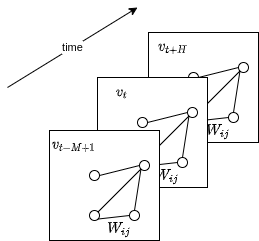
\includegraphics{./images/base.png}
  \centering
  \caption{
نمایش رابطه \رجوع{eq:base} به صورت شهودی.
گراف مسیر یکسان است و هر دیاگرام نشان‌دهنده‌ی سرعت ترافیک در گره‌های این گراف در یک لحظه متفاوت است.
}
  \label{fig:base}
\end{figure}

\پاراگراف{}
بدیهی است تغییر سرعت ترافیک در یک گره‌ی گراف می‌تواند باعث تغییر سرعت ترافیک در گره‌های مجاور شود و هر چه فاصله‌ی دو گره از یک دیگر کم تر باشد این اثرگذاری قوی‌تر است.
برای نمایش این عامل به صورت کمی از ماتریس $W$ استفاده می‌کنیم، ابعاد این ماتریس به صورت $n \times n$ است که $n$ برابر تعداد گره‌های گراف است و هر مقدار داخل این ماتریس تابعی از فاصله‌ی بین دو گره متناظر است که مقدار آن با کاهش این فاصله بیشتر می‌شود.

\پاراگراف{}
در شکل \رجوع{fig:base} $W_{i,j}$ مقدار ماتریس $W$ در خانه‌ی $i$ و $j$ است که نشان دهنده‌ی میزان ارتباط مکانی و همبستگی بین گره‌های $i$ و $j$ می‌باشد.
در این مثال گره‌های $i$ و $j$ همان میادین یاد شده هستند و $W_{i,j}$ با توجه به فاصله‌ی مکانی این دو میدان نشان می‌دهد که
به طور مثال اگر سرعت ترافیک در میدان فاطمی کاهش پیدا کند این موضوع چقدر می‌تواند بر روی سرعت ترافیک در میدان فلسطین تاثیر بگذارد.
در این پروژه از رابطه‌ \رجوع{eq:distance} برای بدست آوردن خانه‌های ماتریس $W$ استفاده می‌کنیم \مرجع{1709.04875}:

\begin{equation}
  W_{i,j} = \left\{
    \begin{array}{ll}
      \exp(-\frac{d^{2}_{ij}}{\sigma^{2}}) & , i \neq j \quad and \quad \exp(-\frac{d^{2}_{ij}}{\sigma^{2}}) \geq \epsilon \\
      0 & , otherwise. \\
    \end{array}\right.
  \label{eq:distance}
\end{equation}

\begin{table}[h]
  \centering
  \caption{توضیح پارامترهای رابطه \رجوع{eq:distance}}
  \begin{tabular}{|c|p{0.5\textwidth}|}
    \hline
    $W_{ij}$ & میزان ارتباط مکانی بین گره‌های $i$ و $j$ \\
    \hline
    $d_{ij}$ & فاصله ی مکانی بین گره‌های $i$ و $j$ \\
    \hline
    $\sigma$, $\epsilon$ & پارامترهای ثابت برای کنترل میزان تنک\پانویس{Sparsity} بودن ماتریس $W$ \\
    \hline
  \end{tabular}
  \label{tbl:distance}
\end{table}

\پاراگراف{}
در مثال ما فاصله بین میدان‌های فاطمی و فلسطین برابر $1.7$ کیلومتر است.
هرچه $\epsilon$ را افزایش دهیم باعث می‌شود تنها ارتباطات قوی‌تر را به حساب بیاوریم و ماتریس تنک‌تر می‌شود
همچنین هرچه $\sigma$ را کاهش دهیم عددی که به عنوان میزان ارتباط محاسبه می‌کنیم کاهش یافته و ماتریس تنک‌تر می‌شود.

\پاراگراف{}
با توجه به توضیحات بالا برنامه توسعه‌یافته‌ی نهایی بر اساس این مدل برای عملکرد به دو فایل ورودی احتیاج دارد که اطلاعات درج شده در شکل \رجوع{fig:blackbox} را در اختیار برنامه قرار دهند.
فایل اول شامل ماتریس $W$ است که پیشتر توضیح داده شد و گراف یا به عبارتی وزن یال‌ها را شرح می‌دهد،
فایل دیگر شامل سرعت ترافیک در نودهای این گراف در بازه‌های زمانی متوالی قرار می‌گیرد $(V_{t}, \ldots, V_{t-M+1})$.
در خروجی، سرعت ترافیک پیش‌بینی شده در نودها در قدم‌های زمانی بعدی برگردانده می‌شود $\hat{V}$.
در مثال ما فایل‌های ذکر شده فرمتی مانند جدول \رجوع{tbl:speed-example} و \رجوع{tbl:distance-example} دارند البته اعداد زیر به صورت تصادفی و فرضی هستند.

\begin{figure}
  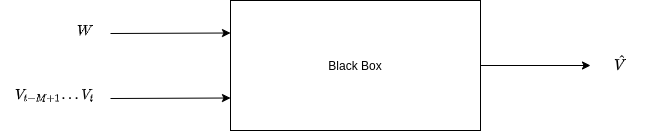
\includegraphics[height=3cm]{./images/blackbox.png}
  \centering
  \caption{
در یک نگاه سطح بالا برنامه با دانستن گراف و سرعت ترافیک در گره‌های این گراف در $M$ واحد زمانی گذشته سرعت ترافیک در $H$ واحد زمانی بعدی را تخمین زده و برمی‌گرداند.
  }
  \label{fig:blackbox}
\end{figure}

\شروع{لوح}[h]
\شرح{مثالی از فرمت فایل ورودی برنامه که شامل سرعت ترافیک در میادین فلسطین و فاطمی در سه قدم زمانی است.}
\تنظیم‌ازوسط
\برچسب{tbl:speed-example}
\شروع{جدول}{|c|c|c|c|}
\خط‌پر
۲ بعد از ظهر & ۱:۵۵ بعد از ظهر & ۱:۵۰ بعد از ظهر & \\
\خط‌پر
۳۶ کیلومتر بر ساعت & ۳۲ کیلومتر بر ساعت & ۴۰ کیلومتر بر ساعت & میدان فلسطین \\
\خط‌پر
۱۷ کیلومتر بر ساعت & ۲۷ کیلومتر بر ساعت & ۱۰ کیلومتر بر ساعت & میدان فاطمی \\
\خط‌پر
\پایان{جدول}
\پایان{لوح}

\شروع{لوح}[h]
\شرح{مثالی از فرمت فایل ورودی برنامه که شامل وزن یالها برای نشان دادن میزان ارتباط مکانی است.}
\تنظیم‌ازوسط
\برچسب{tbl:distance-example}
\شروع{جدول}{|c|c|c|}
\خط‌پر
میدان فاطمی & میدان فلسطین & \\
\خط‌پر
۳۱۶ & ۰ & میدان فلسطین \\
\خط‌پر
۰ & ۳۱۶ & میدان فاطمی \\
\خط‌پر
\پایان{جدول}
\پایان{لوح}


\پاراگراف{}
برای سادگی گراف را بدون جهت در نظر می‌گیریم و در نتیجه $W$ ماتریسی متقارن است.

\پاراگراف{}
برنامه برای آنکه بتواند هم ارتباطات مکانی و هم ارتباطات زمانی را یاد بگیرد باید از بلوک‌هایی تشکیل شده باشد که هر دو نوع لایه پیچشی زمانی و مکانی را در خود داشته باشند.
همانطور که در شکل \رجوع{fig:blocks} نشان داده شده است، ساختار برنامه از دو بلوک پیچشی زمانی-مکانی و یک لایه‌ی خروجی کاملا متصل در انتها تشکیل شده است.

\begin{figure}
  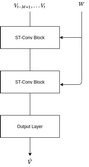
\includegraphics[height=8cm]{./images/blocks.png}
  \centering
  \caption{
شبکه‌ی پیچشی زمانی-مکانی بر روی گراف \مرجع{1709.04875}
  }
  \label{fig:blocks}
\end{figure}

\پاراگراف{}
هر بلوک پیچشی زمانی-مکانی که در شکل \رجوع{fig:inner-blocks} نشان داده شده است از دو لایه‌ی پیچشی زمانی تشکیل شده است که در ورودی و خروجی قرار گرفته‌اند
و یک لایه‌ی پیچش مکانی گراف مانند پلی بین آن دو قرار گرفته است، که می‌تواند با سرعت خوبی اطلاعات مکانی را پس از اعمال پیچش روی گراف
به پیچش‌های زمانی انتشار دهد.

\begin{figure}
  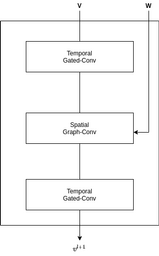
\includegraphics[height=8cm]{./images/inner-blocks.png}
  \centering
  \caption{
ساختار بلوک پیچشی زمانی-مکانی. گراف مسیرها تنها در لایه‌ی پیچش مکانی گراف استفاده می‌شود. \مرجع{1709.04875}
  }
  \label{fig:inner-blocks}
\end{figure}

\پاراگراف{}
در این پروژه برای استخراج ویژگی‌های مکانی از پیچش روی گراف استفاده می‌کنیم و بدیهی است پیچش استاندارد که معمولا
در بحث پردازش تصویر روی تصاویر اعمال می‌کنیم در این مساله قابل استفاده نیست
چرا که در پردازش تصویر پیچش عملا کار الگویابی\پانویس{Pattern Matching} را انجام می‌دهد اما در گراف که رئوس جای مشخصی ندارد
و راس‌های یک گراف را می‌توان به صورت‌های مختلفی
شماره‌گذاری کرد نمی‌توان از پیچش انتظار الگویابی داشت.
و باید از مدل عمومی‌تری استفاده کنیم.

\پاراگراف{}
در پردازش تصویر از کرنل‌هایی مانند شکل \رجوع{fig:2d-convolution} استفاده می‌شود. تمامی خانه‌ها همواره در جای مشخص خود و با ترتیب ثابت قرار گرفته‌اند
برای مثال خانه‌ی $j3$ همیشه در گوشه بالا قرار گرفته است.

\begin{figure}
  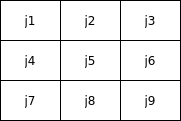
\includegraphics[]{./images/2d-convolution.png}
  \centering
  \caption{کرنل پیچش دو بعدی}
  \label{fig:2d-convolution}
\end{figure}

\پاراگراف{}
می‌خواهیم کرنل شکل \رجوع{fig:graph-convolution-kernel}
به گراف شکل \رجوع{fig:graph-convolution-graph} اعمال کنیم و واضح است که یک نام‌گذاری با ترتیب یکسان برای گراف و کرنل وجود ندارد.


\begin{figure}
  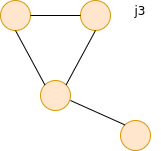
\includegraphics[]{./images/graph-convolution-kernel.png}
  \centering
  \caption{کرنل پیچش گراف}
  \label{fig:graph-convolution-kernel}
\end{figure}

\begin{figure}
  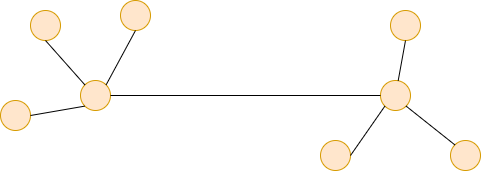
\includegraphics[]{./images/graph-convolution-graph.png}
  \centering
  \caption{گراف مقصد پیچش گراف}
  \label{fig:graph-convolution-graph}
\end{figure}

\پاراگراف{}
در این پژوهش از پیچش طیفی روی گراف‌\پانویس{Spectral Graph Convolution} استفاده می‌کنیم. \مرجع{1312.6203}

\پاراگراف{}
با استفاده از رابطه \رجوع{eq:convolution} می‌توانیم پیچش روی گراف را انجام دهیم تا الگوها و ویژگی‌های با معنی را در دامنه‌ی فضا پیدا کنیم.

\begin{equation}
  \Theta *_{g} \chi = \Theta(L)\chi = \Theta(U \Lambda U^{T})\chi = U\Theta(\Lambda)U^{T}\chi
  \label{eq:convolution}
\end{equation}

\begin{table}[h]
  \centering
  \caption{توضیح پارامترهای رابطه \رجوع{eq:convolution}}
  \begin{tabular}{|c|p{0.5\textwidth}|}
    \hline
    $*_{g}$ & عامل پیچش مکانی روی گراف \\
    \hline
    $\chi$ & سیگنال گراف که در این مدل خروجی لایه‌ی پیچش زمانی اول است \\
    \hline
    $\Theta$ & کرنل \\
    \hline
    $L$ & ماتریس لاپلاسین نرمال شده‌ی گراف \\
    \hline
    $U$ & ماتریس بردار ویژه‌های ماتریس $L$ \\
    \hline
    $\Lambda$ & ماتریس قطری مقدار ویژه‌های ماتریس $L$ \\
    \hline
  \end{tabular}
  \label{tbl:distance}
\end{table}

\پاراگراف{}
در مثال ذکر شده اگر محاسبات را انجام دهیم، خواهیم داشت:

\[
U = \left(
  \begin{array}{cc}
  1 & -1 \\
  1 & 1 \\
  \end{array}
\right),
\Lambda = \left(
  \begin{array}{cc}
  0 & 0 \\
  0 & 2 \\
  \end{array}
\right),
L = \left(
  \begin{array}{cc}
  1 & -1 \\
  -1 & 1 \\
  \end{array}
\right)
\]

در نظر داشته باشید که المان‌های ماتریس $\Theta$ در ابتدا به صورت تصادفی انتخاب می‌شوند.

\پاراگراف{}
پیچیدگی زمانی این رابطه $O(n^{2})$ است که بسیار سنگین است برای سبک شدن محاسبات باید از یک تخمین به جای استفاده مستقیم از این رابطه بهره ببریم.
در این پروژه از تخمین چند جمله‌ای چبیشف\پانویس{Chebyshev} استفاده می‌کنیم.

\پاراگراف{}
برای متمرکز و محلی کردن فیلتر و کاهش تعداد پارامترها، می‌توان کرنل $\Theta$ را به یک چند جمله‌ای از $\varLambda$ محدود کرد.

\[
  \Theta(\varLambda) = \sum_{k=1}^{k-1}\Theta_{k}\varLambda^{k}
\]

$k$ اندازه کرنل در پیچش گراف است که شعاع بیشینه پیچش از یک گره مرکزی را مشخص می‌کند. از چند جمله‌ای چبیشف $T_{k}(x)$ استفاده می‌کنیم تا
کرنل‌ها را به صورت انبساطی کوتاه شده از مرتبه‌ی $k-1$ تخمین بزنیم.

\[
  \Theta(\varLambda) \approx \sum_{k=1}^{k-1}\Theta_{k}T_{k}(\widetilde{\varLambda})
\]
\[
  \widetilde{\varLambda} = \frac{2\widetilde{\varLambda}}{\lambda_{\max}} - I_{n}
\]

حال می‌توانیم پیچش روی گراف را اینگونه بازنویسی کنیم:

\begin{equation}
  \Theta \ast_{g} x = \Theta(L)x \approx \sum_{k=0}^{k-1} \Theta_{k} T_{k}(\widetilde{L})x
  \label{eq:approx-convolution}
\end{equation}

$T_{k}(\widetilde{L} \in R^{n \times n})$ چند جمله‌ای چبیشف از مرتبه‌ی $k$ است که به وسیله‌ی لاپلاس اسکیل شده محاسبه می‌شود.

\[
  \widetilde{L} = \frac{2\widetilde{L}}{\lambda_{\max}} - I_{n}
\]

از تقریب چند جمله‌ای استفاده می‌کنیم و به طور بازگشتی $k$ پیچش‌های محلی را محاسبه می‌کنیم. اینگونه می‌توانیم رابطه‌ی \رجوع{eq:convolution}
را با رابطه‌ی \رجوع{eq:approx-convolution} تخمین بزنیم و پیچیدگی محاسباتی را از $O(n^{2})$ به $O(k|\epsilon|)$
کاهش دهیم.

\پاراگراف{}
در مسائل سری زمانی، شبکه‌های عصبی بازگشتی بسیار رایج‌اند اما در مسایل ترافیک استفاده از این شبکه‌ها بسیار زمان‌بر است.
همچنین در ترافیک تغییرات به صورت پویا می‌باشند که این شبکه دیر به این تغییرات جواب می‌دهد،
در طرف دیگر شبکه های عصبی پیچشی به سرعت آموزش داده می‌شوند و ساختار ساده‌ای دارند، در نتیجه برای استخراج ویژگی‌های زمانی در این پروژه با الهام از
\مرجع{1409.3215} از ساختارهای کاملا پیچشی بر روی محور زمان استفاده می‌کنیم تا بتوانیم رفتار پویای سرعت ترافیک را دنبال کنیم.

\begin{figure}
  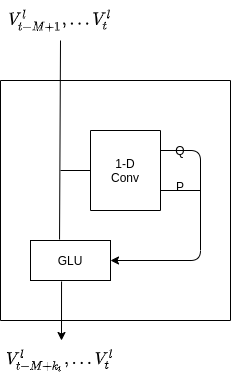
\includegraphics[height=8cm]{./images/time-conv.png}
  \centering
  \caption{
ساختار لایه‌ی کانولوشنی زمانی \مرجع{1709.04875}
  }
  \label{fig:time-conv}
\end{figure}

\پاراگراف{}
شکل \رجوع{fig:time-conv} لایه‌ی پیچشی زمانی را نشان می‌دهد که شامل یک پیچش علّی یک بعدی\پانویس{1-D casual convolution}
با یک فیلتر به عرض  $k_{t}$ است که پس از آن یک \متن‌لاتین{Gated Linear Unit} قرار دارد.
برای هر گره در گراف $g$ پیچش زمانی بر روی تمامی $K_{t}$ همسایه‌ی ورودی اعمال می‌شود.
در این پیچش لایه گذاری\پانویس{padding} وجود ندارد‌‌، در نتیجه، پیچش در هر مرتبه باعث کوتاه‌تر شدن توالی‌ها به اندازه‌ی $K_{t}-1$ می‌شود.
با این توضیحات می‌توانیم رابطه‌ی \رجوع{eq:time-conv} را بیان کنیم.

\begin{equation}
  \Gamma *_{\tau} Y = P \odot \sigma (Q) \in R^{M-K_{t}+1 \times C_{O}}
  \label{eq:time-conv}
\end{equation}

\begin{table}[h]
  \centering
  \caption{توضیح پارامترهای رابطه \رجوع{eq:time-conv}}
  \begin{tabular}{|c|p{0.5\textwidth}|}
    \hline
    $*_{g}$ & عامل پیچش زمانی \\
    \hline
    $Y$ & سرعت ترافیک در گره‌های مختلف گراف در گام‌های زمانی گذشته \\
    \hline
    $\Gamma$ & کرنل پیچش که المان‌های آن در ابتدا به صورت تصادفی انتخاب می‌شوند. \\
    \hline
    $P$, $Q$ & پس از آنکه با استفاده از کرنل $\Gamma$ یک پیچش روی $Y$ اعمال کردیم خروجی را برحسب سایز کانال خروجی لایه به دو نیمه‌ی مساوی تقسیم می‌کنیم که یکی $P$ و دیگری را $Q$ می‌نامیم. \\
    \hline
    $\odot$ & نمایشگر عملیات ضرب درایه‌ای \\
    \hline
    $M$ & تعداد گام‌های زمانی استفاده شده برای آموزش \\
    \hline
    $K_{t}$ & سایز کرنل \\
    \hline
    $C_{O}$ & سایز کانال خروجی \\
    \hline
  \end{tabular}
  \label{tbl:distance}
\end{table}

\پاراگراف{}
 $P$ و $Q$ پس از محاسبه به عنوان ورودی به \متن‌لاتین{Gated Linear Unit} داده می‌شوند، این واحد باعث غیرخطی شدن محاسبات این لایه می‌شود.

\پاراگراف{}
ورودی $Y$ چهار بعدی است، بُعد اول برابر تعداد کل داده‌هایی است که در اختیار داریم، بُعد دوم برابر
تعداد گام‌های گذشته است، که قصد داریم برای پیش‌بینی استفاده کنیم،
بُعد سوم برابر تعداد گره‌های گراف و در نهایت بُعد آخر سایز کانال ورودی است.
در مثالی که با آن پیش می‌رویم تعداد کل داده‌ها سه، تعداد گام‌های زمانی گذشته مورد استفاده برای پیش‌بینی مدل برابر دو،
تعداد گره‌های گراف برابر دو و سایز کانال ورودی برابر یک است، در نتیجه ابعاد $Y$ به صورت $ 3 \times 2 \times 2 \times 1 $ در میاید.

\پاراگراف{}
همانطور که پیش‌تر اشاره شد در این پیچش لایه‌گذاری وجود ندارد در نتیجه ابعاد خروجی این لایه مانند ابعاد ورودی است به جز بعد دوم
که پس اعمال پیچش به اندازه‌ی $K_{t}-1$ کاهش میابد. حال اگر عرض $K_{t}$ را در مثالمان برابر ۲ در نظر بگیریم
بعد دوم ورودی به اندازه‌ی ۱ واحد کوچکتر و برابر با ۱ می‌گردد.

\پاراگراف{}
از آنجایی که مقادیر کرنل $\Gamma$ تصادفی می‌باشند، ادامه مثال ارزش افزوده‌ای نداشته بنابراین به آوردن مثال تا به این نقطه بسنده می‌کنیم.

\پاراگراف{}
در نهایت بلوک‌های پیچش زمانی-مکانی از رابطه \رجوع{eq:blocks} پیروی می‌کنند که در آن $L_{0}$ و $L_{1}$ به ترتیب کرنل‌ لایه‌های پیچشی زمانی پایینی و بالایی و $\Theta$ کرنل پیچش مکانی روی گراف می‌باشد.

\begin{equation}
v^{{l+1}} = \Gamma^{l}_{1} *_{\tau} ReLU( \Theta^{l} *_{g} (\Gamma_{0}^{l} *_{\tau} v^{l}) )
  \label{eq:blocks}
\end{equation}

بعد از روی هم قرار دادن دو بلوک پیچش زمانی-مکانی یک لایه‌ی کاملا متصل به عنوان لایه‌ی خروجی در انتها قرار می‌دهیم (مطابق شکل \رجوع{fig:blocks}).

\قسمت{ابزارها و امکانات مورد نیاز}
مرتبه زمانی روش پیچش روی گراف به این دلیل که امکان استفاده از تبدیل سریع فوریه\پانویس{FFT} وجود ندارد،
\[
O(n^{2})
\]
می‌باشد و اعمال این روش بدون داشتن تجهیزات گران قیمتی مانند پردازنده‌های گرافیکی زمان قابل توجهی است. حداقل امکانات مورد نیاز برای اجرای این پروژه عبارت اند از:

\begin{latin}\begin{itemize}
\item CPU: Intel(R) Xeon(R) CPU E5-2620 v4 @ 2.10GHz
\item GPU: NVIDIA GeForce GTX 1080
\end{itemize}\end{latin}

\قسمت{ارزیابی}
در نهایت به منظور ارزیابی پروژه از داده‌های ترافیکی واقعی \متن‌لاتین{PeMSD7} استفاده می‌کنیم که توسط اداره‌ی حمل و نقل ایالت کالیفرنیا\پانویس{https://pems.dot.ca.gov/} جمع آوری شده است.
این داده مربوط به ۲۲۸ ایستگاه می‌باشد که به صورت تصادفی از میان ۳۹ هزار ایستگاه‌ انتخاب شده‌اند و شامل ۱۲ هزار سطر است که نشان دهنده‌ی سرعت ترافیک در این ۲۲۸ ایستگاه با توالی زمانی پنج دقیقه می‌باشد.
داده‌ها در ماه‌های می تا جون سال ۲۰۱۲ جمع آوری شده‌اند و جهت پاک کردن داده‌های ترافیکی بی‌قاعده روزهای غیرکاری حذف شده‌اند.
برای مقایسه‌ی عملکرد این روش با روش‌های دیگر از معیارهای میانگین مطلق خطا\پانویس{MAE}، میانگین مطلق درصد خطا\پانویس{MAPE} و جذر میانگین مربعات خطا\پانویس{RMSE} استفاده می‌کنیم.
این روش را با روش‌های پایه‌ی شبکه‌ی عصبی پیش‌خور\پانویس{Feed-Forward Neural Network}، مدل خودهمبسته میانگین متحرک و حافظه‌ی کوتاه مدت ماندگار کاملا متصل\پانویس{Full-Connected LSTM} \مرجع{1409.3215} مقایسه خواهیم کرد.

\قسمت{زمان‌بندی انجام پروژه}

\شروع{لوح}[h]
\تنظیم‌ازوسط
\شروع{جدول}{|c|c|}
\خط‌پر
مدت زمان & فعالیت \\
\خط‌پر
سه ماه & پیاده‌سازی \\
\خط‌پر
یک ماه & آموزش مدل و ارزیابی \\
\خط‌پر
دو ماه & بهبود‌های احتمالی (از نظر مرتبه‌ی زمانی) \\
\خط‌پر
دو ماه & جمع‌بندی \\
\خط‌پر
\پایان{جدول}
\پایان{لوح}

\bibliographystyle{ieeetr}
\bibliography{references}

    \vspace*{\fill}
    \begin{center}
این سند برپایه بسته \متن‌لاتین{\زی‌پرشین} گونه \متن‌لاتین{\گونه‌زی‌پرشین} توسعه پیدا کرده است.
    \end{center}

\end{document}
